%%%%%%%%%%%%%%%%%%%%%%%%%%%%%%%%%%%%%%%%%%%%%%%%%%%%%%%%%%%%%%%
%
% Welcome to Overleaf --- just edit your LaTeX on the left,
% and we'll compile it for you on the right. If you open the
% 'Share' menu, you can invite other users to edit at the same
% time. See www.overleaf.com/learn for more info. Enjoy!
%
%%%%%%%%%%%%%%%%%%%%%%%%%%%%%%%%%%%%%%%%%%%%%%%%%%%%%%%%%%%%%%%


% Inbuilt themes in beamer
\documentclass{beamer}

% Theme choice:
\usetheme{CambridgeUS}

% Title page details: 

\usepackage{polynom}
\usepackage{amssymb}
\usepackage{amsmath}

\usepackage{bm}
\usepackage[misc]{ifsym}
%\setlength{\columnseprule}{1pt}
%\def\columnseprulecolor{\color{blue}}

\usepackage{longtable}
\usepackage{enumitem}
\usepackage{mathtools}
\usepackage[applemac]{inputenc}
\usepackage{tikz}
\usepackage{listings}
    \usepackage{color}                                            %%
    \usepackage{array}                                            %%
    \usepackage{longtable}                                        %%
    \usepackage{calc}                                             %%
    \usepackage{multirow}                                         %%
    \usepackage{hhline}                                           %%
    \usepackage{ifthen}                                           %%
  
\usepackage{lscape}     
\usepackage{tfrupee}
\usepackage{parskip}

\DeclareMathOperator*{\Res}{Res}
\DeclareMathOperator*{\equals}{=}
\DeclareMathOperator*{\pipe}{|}

\hyphenation{op-tical net-works semi-conduc-tor}
\def\inputGnumericTable{}  
\graphicspath{{./images/}}


\begin{document}
\newcommand{\bfr}[2]{\section{#1} \begin{frame}{#1} #2 \end{frame}}

	\title{Assignment 8}
		\author{ Abhay Shankar K : CS21BTECH11001}

	\begin{frame}
    		\titlepage 
	\end{frame}

	\begin{frame}{Outline}
    		\tableofcontents
	\end{frame}

	\providecommand{\brak}[1]{\ensuremath{\left(#1\right)}}
	\providecommand{\sbrak}[1]{\ensuremath{\left[#1\right]}}
	\providecommand{\cbrak}[1]{\ensuremath{\left\{#1\right\}}}
	\providecommand{\req}{\textbf{Required :}}
	\providecommand{\rpr}[2]{\ensuremath{P_{#1}\left(#2\right)}} %random variable notation
	\providecommand{\spr}[1]{\ensuremath{P\left(#1\right)}} %simple notation
	\providecommand{\cpr}[2]{\ensuremath{\spr{#1 \pipe #2}}} %conditional probability
	\newcommand*{\permcomb}[4][0mu]{{{}^{#3}\mkern#1#2_{#4}}}
	\newcommand*{\perm}[1][-3mu]{\permcomb[#1]{P}}
	\newcommand*{\comb}[1][-1mu]{\permcomb[#1]{C}}
	
	\bfr{Question}{
	
	A box contains $n$ identical balls labelled $1$ through $n$. Suppose $k$ balls are drawn in succession. What is the probability that :
	\begin{enumerate}[label = \brak{\textbf{\roman*}}]
	
		\item $m$ is the largest number drawn. (Event A)
		
		\item The largest number drawn is less than or equal to $m$. (Event B)
		
	\end{enumerate}
	
	}

		
	\bfr{Random Variables}{	
	Let the random variable $X$ denote the largest number drawn.
	
	\req 
	
	\begin{enumerate}[label = \brak{\textbf{\roman*}}]
	
		\item \spr{A} = \rpr{X}{m}
	
		\item \spr{B} = $\Sigma_{i = 1}^{m} \rpr{X}{i}$
		
	\end{enumerate}
	}
	
	\bfr{Solution}{
	Let $M$ be the event that $m$ is drawn.
	Clearly, 
	
	\begin{align}
		\spr{A} = \rpr{X}{m} = \spr{MB} 
			\label{form}
	\end{align}	

	Therefore, we shall find \spr{B} first.

	\begin{align}
		\spr{B} &= \frac{\# \text{ Ways of drawing from } \sbrak{m}}{\# \text{ Ways of drawing from } \sbrak{n}} \nonumber \\
			&= \frac{\comb{m}{k}}{\comb{n}{k}} 
				\label{B_soln}
	\end{align}
	}
	
	\bfr{}{
	We know,
		\begin{align}
			\spr{M} = 	\frac{k}{n} \\
			\implies \cpr{B}{M} &= \frac{\# \text{Ways of drawing } i \in \sbrak{m - 1} k - 1 \text{ times}}{\# \text{Ways of drawing } i \in \sbrak{n} - \cbrak{m} k - 1 \text{ times}} \nonumber \\
			&= \frac{\comb{m - 1}{k - 1}}{\comb{n - 1}{k - 1}}
				\label{cond}
		\end{align}
		
		We know $\spr{MB} = \cpr{B}{M} \times \spr{M}$. Thus, substituting ~\eqref{cond} in ~\eqref{form},
		
		\begin{align}
			\spr{A} = \frac{\comb{m - 1}{k - 1}}{\comb{n - 1}{k - 1}} \times \frac{k}{n}
				\label{A_soln}
		\end{align}
			
	}
	
	\bfr{Graphs}{
	\begin{figure}[h!]
		\caption{Graph for event A}
		
		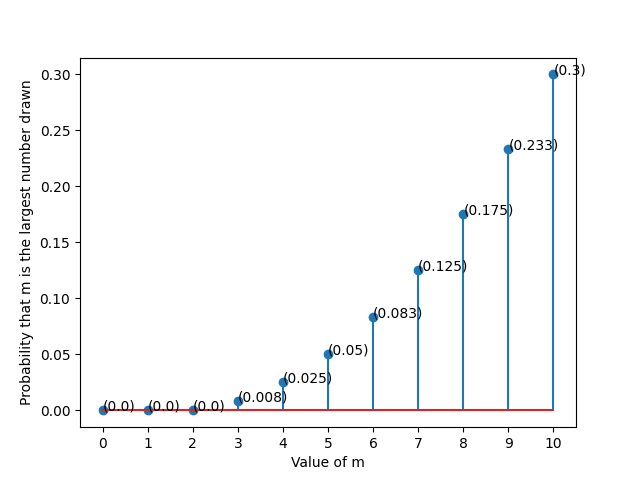
\includegraphics[scale = 0.5]{assig8_pmf}
	\end{figure}
	}
	\bfr{}{
	\begin{figure}[h!]
		\caption{Graph for event B}
		
		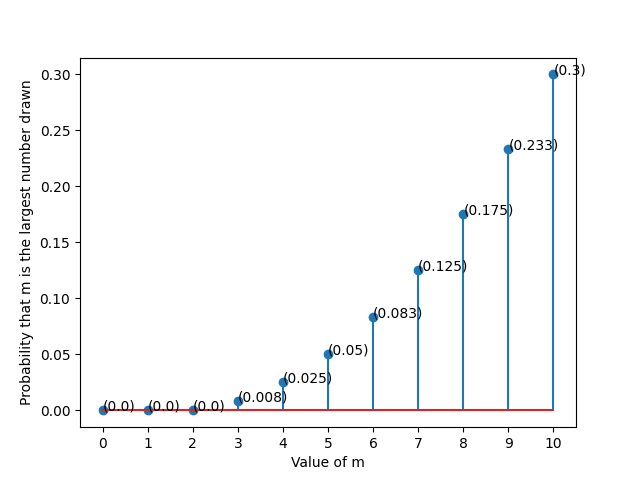
\includegraphics[scale = 0.5]{assig8_pmf}
	\end{figure}

	}
						
\end{document}
	
	

	
	
	
	